\documentclass[a4paper,12pt]{scrartcl}
\usepackage[utf8]{inputenc}
\usepackage[T1]{fontenc}
\usepackage[ngerman]{babel}
\pagestyle{empty}
\usepackage{amsfonts}
\usepackage{amsmath}
\usepackage{graphicx}

\begin{document}

\section{Die Normalverteilung}
Die Normalverteilung, auch Gauß-Verteilung genannt, ist eine der wichtigsten Wahr-\\
scheinlichkeitsverteilungen. Die Dichtefunktion
\begin{equation}
\mathcal{N}(x,\mu,\sigma) = \frac{1}{\sqrt{2\pi\sigma^{2}}} \,{} exp \,{} \bigg(-\frac{(x-\mu)^{2}}{2\sigma^{2}}\bigg)
\end{equation}
wird mit dem Erwartungswert $\mu \,{} \varepsilon \,{} \mathbb{R}$ und der Varianz $\sigma^{2} > 0$ parametrisiert. In\\
Abbildung 1 wird die Gauß-Verteilung im Intervall $x \,{} \varepsilon \,{} [-5,5]$ für die Parameterpaare\\\\
\centerline{$(\mu,\sigma) \,{} \varepsilon \,{} \{(0,0.2),(0,1),(0,5),(-2,0.5)\}$}\\\\
dargestellt.
\begin{figure}[h]
\begin{center}
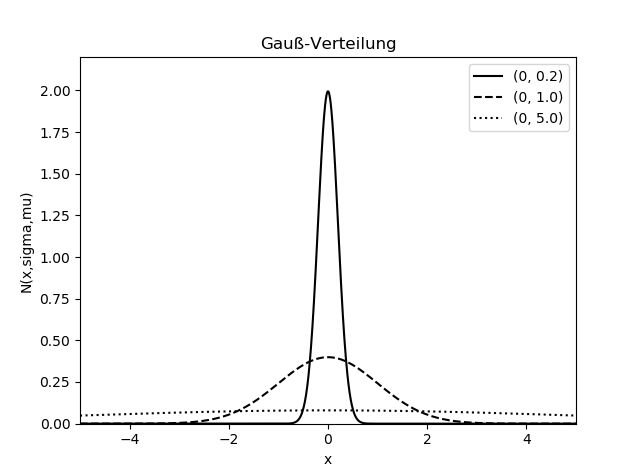
\includegraphics[width=12cm]{GV.jpg}
\caption{Die Gauß-Verteilung aus (1) für $(\mu,\sigma) \,{} \varepsilon \,{} \{(0,0.2),(0,1),(0,5),(-2,0.5)\}$}
\label{latex_logo}
\end{center}
\end{figure}
\end{document}